\section{Results}
We have implemented our method on top of general differentiable renderer\cite{ravi2020accelerating}. 
For all tests, we used Intel Xeon E5-2687W CPU machine with 3.0GHz, and GeForce RTX 2080 TI for CUDA-optimized differentiable renderer. 
We optimized our mesh with Stochastic Gradient Descent method with learning rate = 1.0, and momentum = 0.9. 
For $\mathcal{M}$, we pre-computed from popular off-line SLAM framework \cite{zhou2018open3d} with voxel size 2cm.
We placed one virtual light source at the camera center for all experiments, although this method is up to a number of lights and its positions.


\subsection{Validation of Proposed Method}

\paragraph{Validation of loss}
In (Fig. \ref{fig:loss_plot_with_images}), we plotted our loss graph to ensure that our loss function forms a convex function. 
Our proposed lightweight loss is monotonically decreased as the optimization continues. 
Note that our positional loss is not minimized, as we want positional loss to act similar with regularization term, which prevents evolving vertices getting not to far from its original position. 
Nevertheless, the total loss forms a convex function as the actual contribution of positional loss is small enough than lightweight loss. 
We showed the effect of positional loss in (Fig. \ref{fig:ablation_study_positional_loss}).

\begin{figure}
    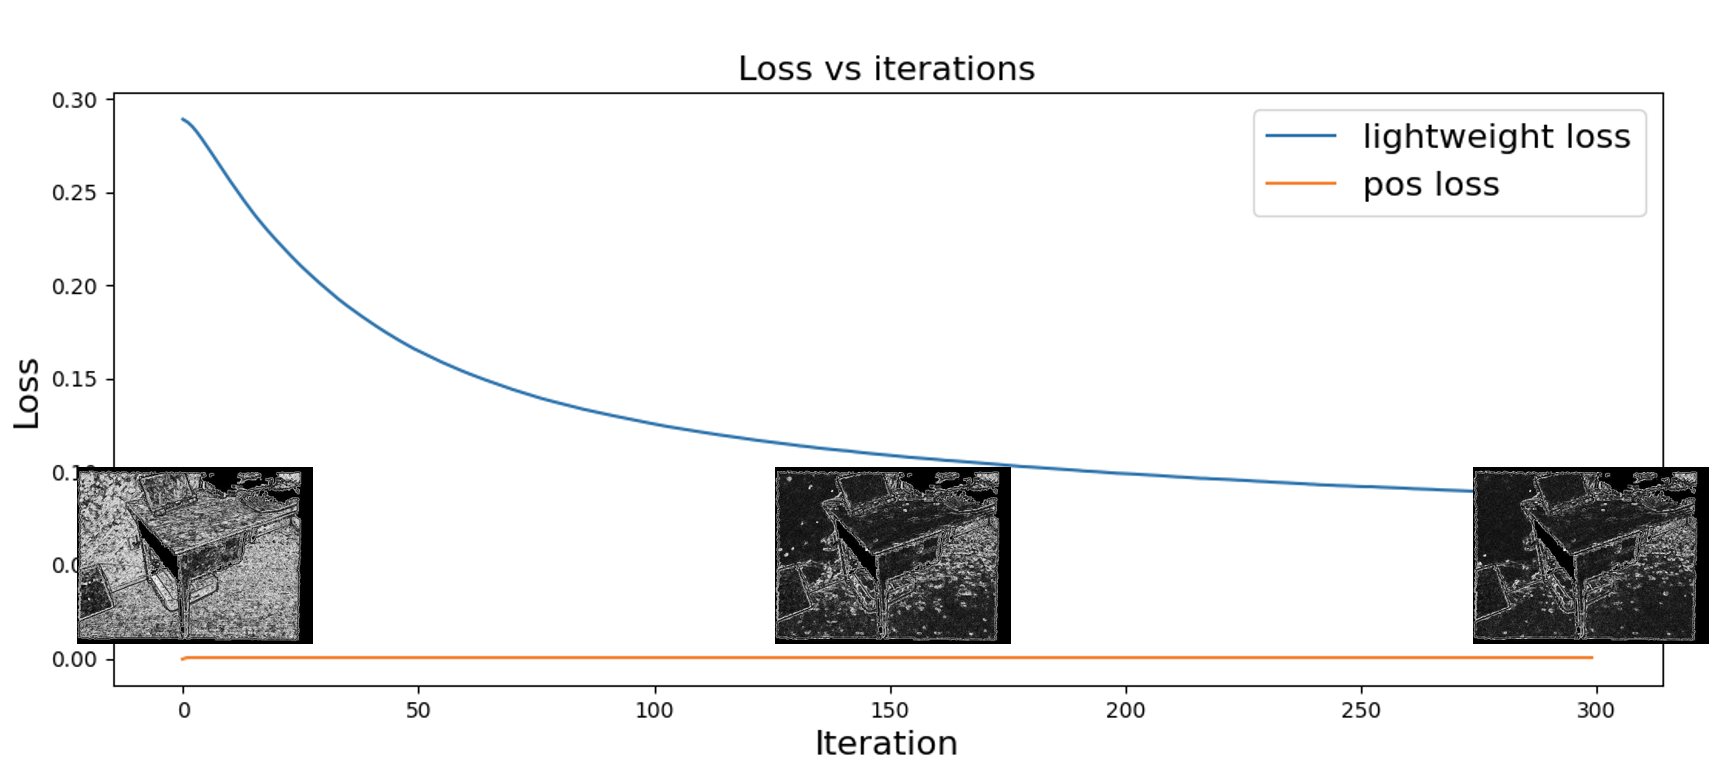
\includegraphics[width=\columnwidth]{figures/4_result_loss_plot_with_images.png}
    \caption{Loss plot with loss images at specific iterations (here, 0, 150, and 300 is used). Our lightweight loss successfully minimizes vertex noise by observing target noise-free geometric information $G_\mathcal{C}$. Note that $L_{pos}$ never converges to zero, as they act as constraint to vertices not to evolve too far from its original position, thus have non-zero values among all iterations.}
    \label{fig:loss_plot_with_images}
\end{figure}

\begin{figure}
    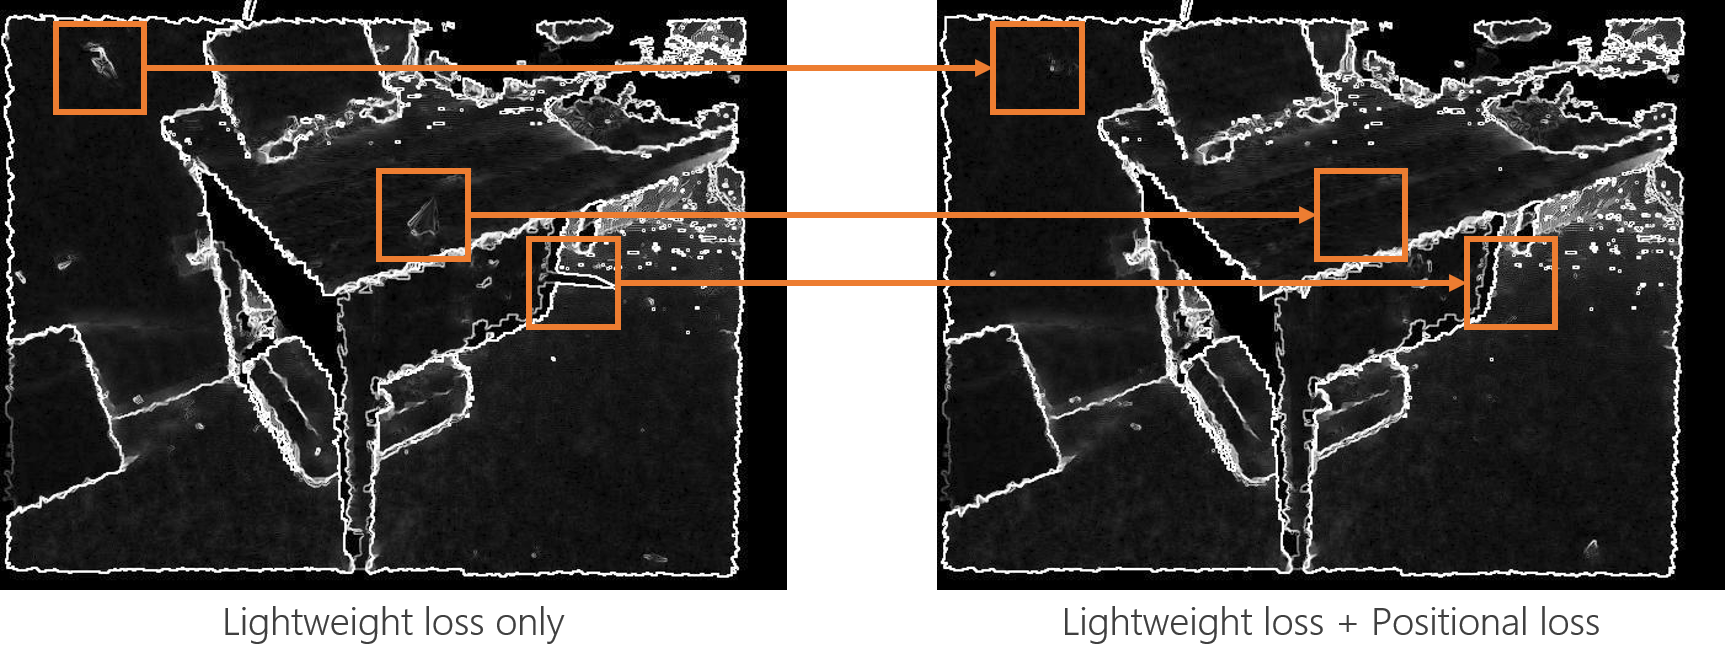
\includegraphics[width=\columnwidth]{figures/4_result_ablation_study_positional_loss.png}
    \caption{Ablation study of positional loss, without loss and with loss, respectively. \textcolor{Orange}{\textbf{Orange}} inset highlights difference of vertex evolving aspect. Note that total loss of both result is converged. (Left) Some vertices are evolved in a wrong direction with respect to its perceived shape (Right) Our result with positional loss successfully maintain its shape, as the loss prevent vertices evolve not too far from its original position.}
    \label{fig:ablation_study_positional_loss}
\end{figure}

\paragraph{Validation with various scenes}
We validated performance of our proposed method, by evaluating minimum eigenvalue of the region where we are able to perceive as 'flat', given $\mathcal{C}$.

\begin{figure}
    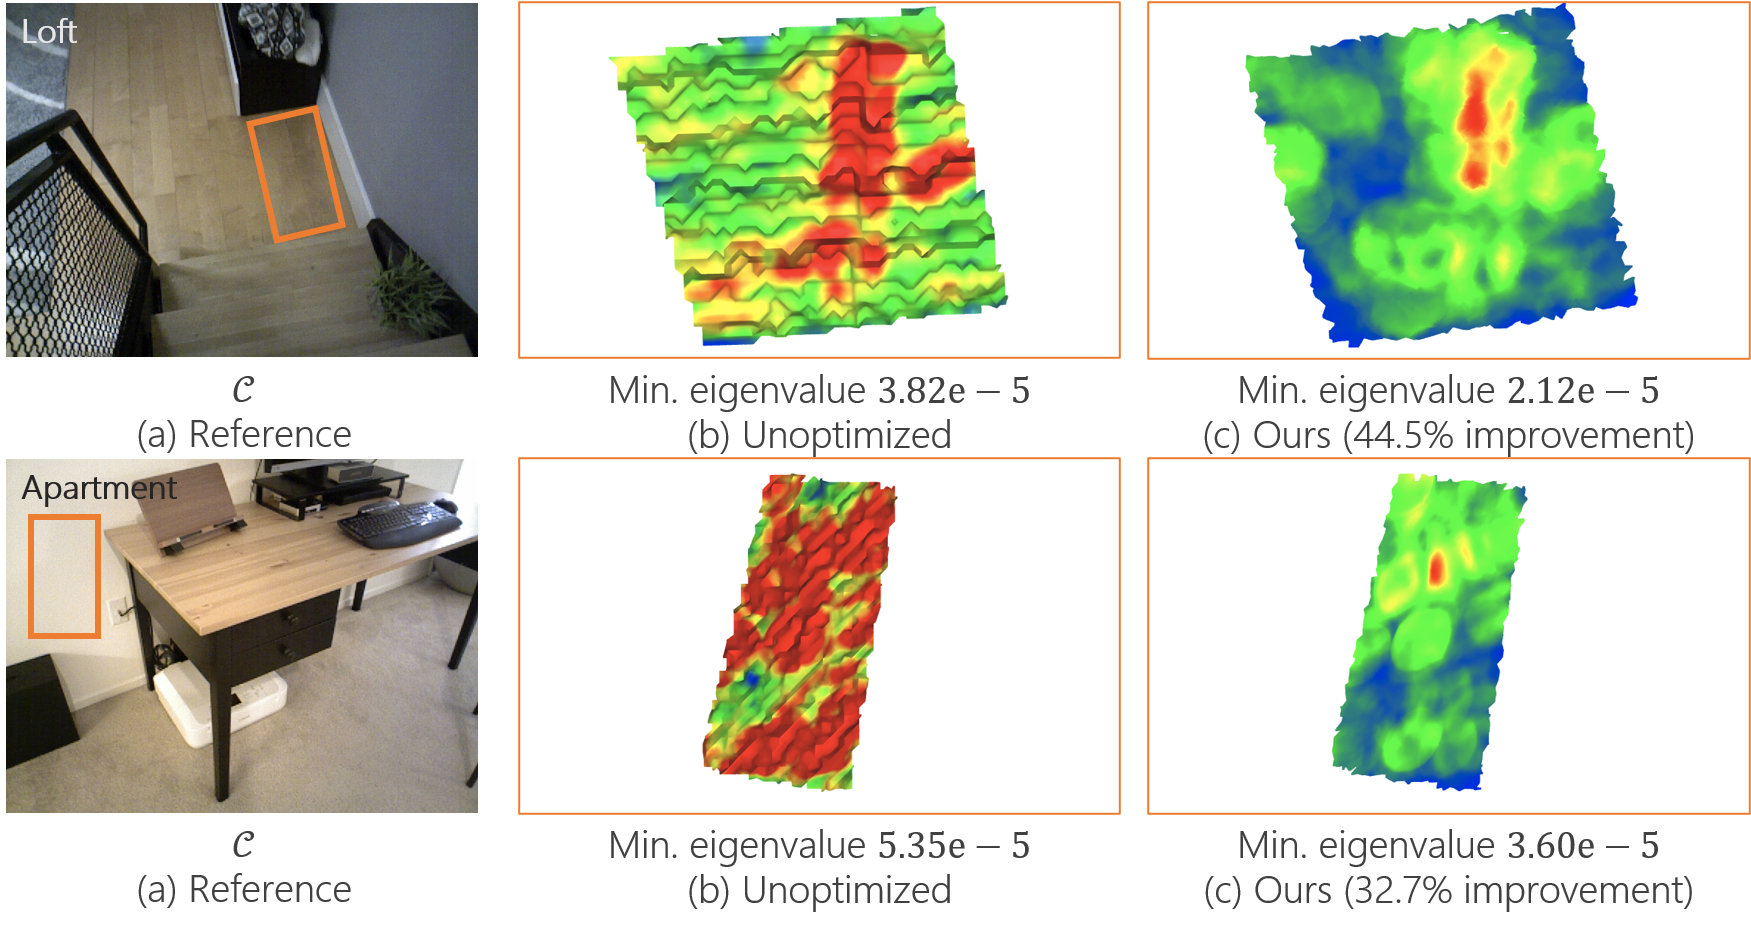
\includegraphics[width=\columnwidth]{figures/4_result_plane_fitting.png}
    \caption{Plane fitting validation of our result. Given scenes, we selected \textcolor{Orange}{\textbf{Orange}} region where is considered as "perceptually flat". We compared minimum eigenvalue between inset of input mesh (Middle) and optimized mesh (Right), and plotted heatmap of each result. Our method successfully minimize minimum eigenvalue within plane.}
\end{figure}

\begin{figure*}
    \centering
    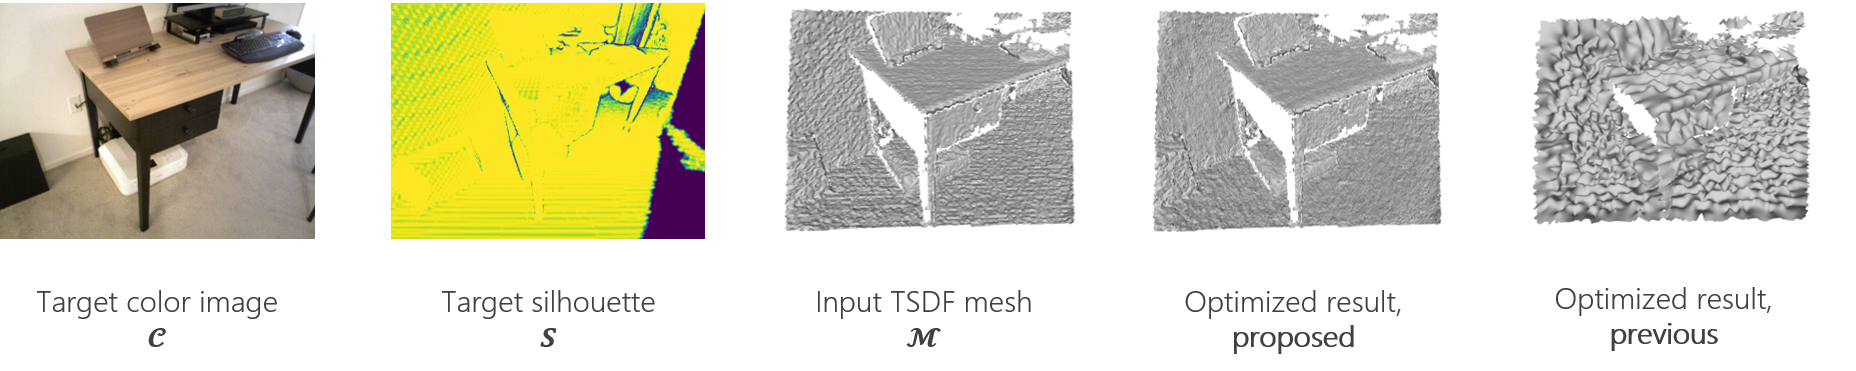
\includegraphics[width=\textwidth]{figures/4_result_comparison_with_previous_method.png}
    \caption{Comparison of result using previous method and our method. For target silhouette, we generated it from input mesh by render mesh with silhouette renderer, and it is enough to use since silhouette image itself does not hold any depth information other than boundary information of target mesh. \textbf{Previous} result fails to converge to perceptive geometric shape hidden in target images, whereas \textbf{Proposed} result successfully reduces noise. Note that \textbf{Proposed} method only observes $\mathbf{\mathcal{C}}$ in order to infer noise-free geometry, whereas Previous method requires both $\mathbf{\mathcal{C}}$ and $\mathbf{S}$.}
    \label{fig:comparison_with_previous_method}
\end{figure*}

\subsection{Comparison with Previous Work}
We compare our method with standard differentiable rendering approach used in differentiable renderer\cite{liu2019soft}. 
We slightly modified its workflow in order to evaluate performance under identical conditions (please refer \ref{fig:difference_simple_mesh_and_tsdf_mesh} for details). 
Specifically, we limit amount of target view to 1, as it is impossible to synthetically generate clean target using existing SLAM sequences. 
For silhouette image, we used silhouette of input TSDF mesh as silhouette itself does not take into account detailed depth information as they represent boundary of mesh \PJ{TODO: to footnote}(Hence, previous methods required silhouette images from different camera extrinsic in order to optimize the shape of input mesh). 
We follow losses and its weights as suggested in previous method\cite{ravi2020accelerating}, which is defined as: 
\begin{multline*}
    \mathcal{L}_{prev}=w_{sil}\cdot L_{sil}+w_{rgb}\cdot L_{rgb}+w_{edge}\cdot L_{edge}+ \\ 
    w_{normal}\cdot L_{normal}+w_{laplacian}\cdot L_{laplacian}, 
\end{multline*}
where $L_{sil}$, $L_{rgb}$ is silhouette, and color difference between input and target, respectively. 
$L_{edge}$, $L_{normal}$, and $L_{laplacian}$ stands for mesh edge length consistency, mesh normal orientation consistency, and mesh Laplacian loss, respectively. 
Note that mesh losses $L_{edge}$, $L_{normal}$, $L_{laplacian}$ is developed from traditional geometry processing field, thus they do not reflect geometric features that are shown in target images. 
For brevity, we skip detailed equations for each loss. 
We used $w_{sil}=1.0$, $w_{rgb}=1.0$, $w_{edge}=1.0$, $w_{normal}=0.01$, $w_{laplacian}=1.0$ as authors suggested.
Fig. 5 shows optimized mesh with loss from previous work. 
Resulting mesh preserves its silhouette information, as they provided silhouette loss to prevent vertices to evolve out of its silhouettes. 
However, vertices within silhouette images are evolved without any shape constraints supervised by target images. 
Those vertices are guided to satisfy input mesh’s internal properties, as mesh losses does not consider geometric clues in target images. 
This results in optimized mesh failed to optimize, while only preserving boundary.

\subsection{Limitations \& Future Directions}
We summarize future directions of our method, including failure case and promising extension of proposed method.
\paragraph{Adding Robust Positional Constraint Loss}
Although our method can drastically reduce mesh noise, we found that optimized mesh is not maintaining topologically correct structure. 
Specifically, we observed self-intersections between neighboring faces. 
This problem can be naturally arisen since we did not consider relationship between neighboring vertices in our final loss. 
Therefore, though vertices are evolved to have reduced noise, their evolving direction is totally random, lead to occur self-intersections between neighboring faces by corresponding (incorrectly evolved) neighboring vertices. 
We illustrated this failure case in Figure 7.


\begin{figure}
    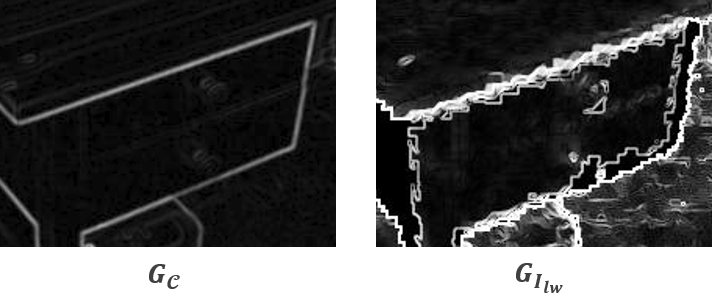
\includegraphics[width=\columnwidth]{figures/4_future_edge_fitting.png}
    \caption{Inset of each gradient. $G_{lw}$ is corrupted since geometric normal deviates around edge.}
    \label{fig:edge_fitting}
\end{figure}


\begin{figure*}
    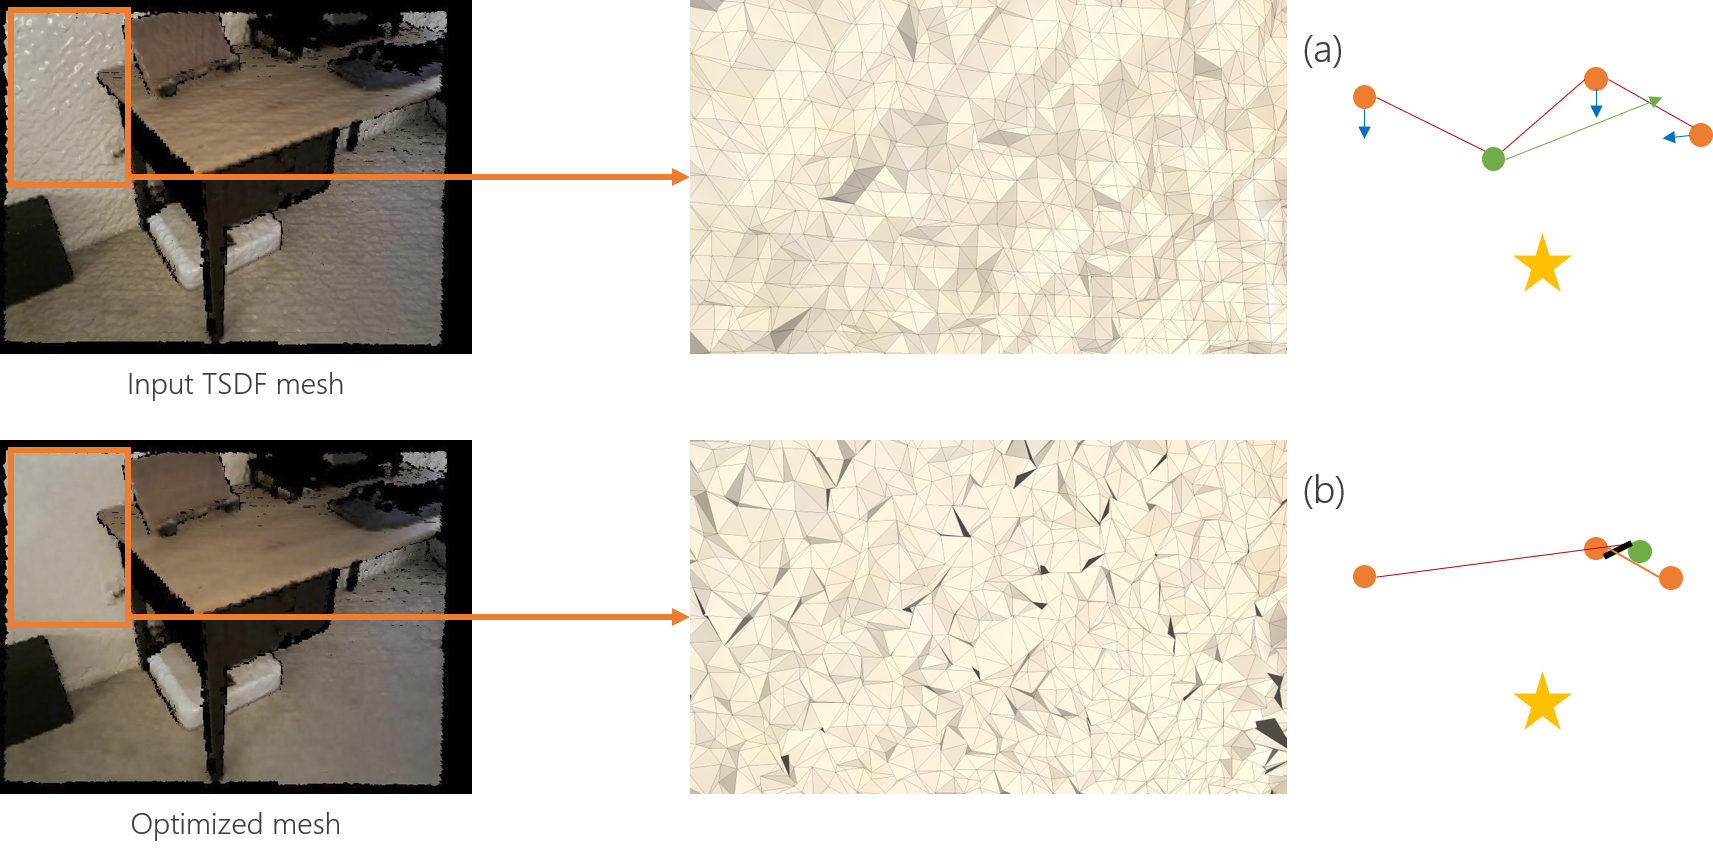
\includegraphics[width=\textwidth]{figures/4_future_work_self_intersection.png}
    \caption{Comparison of input mesh and optimized mesh. We zoomed up each geometry corresponds to image inset. 
    \textbf{Black artifacts} are observed in zoomed view in optimized mesh. We found that those are self-intersection between neighboring faces, since our positional constraint $L_{pos}$ does not consider distances between neighboring vertices. 
    This phenomenon is illustrated at the rightmost images of each zoomed view. 
    (a) For each iteration, vertices are optimized while only considering flatness of surfaces, not for topological correctness of geometry. 
    Star, circle, and arrow indicates light position, vertices, and gradient (evolving direction after current optimization step), respectively. 
    Here, \textbf{\textcolor{ForestGreen}{Green vertex}} is optimized to \textbf{\textcolor{ForestGreen}{Green arrow}} direction so that it occludes another face. 
    (b) Consequently, there exists a self-intersection between neighboring faces (\textbf{Black line}) although the entire mesh noise is reduced, resulting self-occluded artifact.}
    \label{fig:self_intersection}
\end{figure*}

\paragraph{Edge Fitting}
Although our method is able to minimize noisy vertices by treating $G_\mathcal{C}$ as noise-free geometric clue, however it failed to clean out noisy vertices around geometric edges. 
We found that there is gradient magnitude difference between two images, as on edges $G_{lw}$ tends to have large deviation since it is the place where geometric normal hugely differs. 
Our current $L_2$ loss of gradients cannot reflect this case, as they are evaluated pixel-by-pixel. 
We visualized this case in Figure 8. 
Weighting color gradients by using gradients from depth, say $G_\mathcal{D}$, or developing an erosion kernel for $G_\mathcal{C}$ to reliably cover $G_{lw}$ seems worth trying.

